\documentclass[twoside,11pt]{reviewresponse}
\usepackage{amsbsy,amssymb,epsfig,bbm,mathrsfs,multirow,amsthm}
\usepackage{amsmath}
\usepackage{cite}
\usepackage{caption}
\captionsetup[figure]{name=Fig.}
\usepackage{graphicx}
\usepackage[english]{babel}
\usepackage{mathtools,xparse}
\usepackage{color}
\usepackage{luatexja}
\usepackage{enumerate}
\usepackage{booktabs}
\usepackage{colortbl}
\usepackage{bbm}
\usepackage{tocbibind}
\usepackage{comment}
\usepackage{lipsum}
\usepackage{leftidx}
\usepackage{diagbox}[2011/11/22]
\usepackage{makeidx}
\usepackage{lipsum}
\usepackage{makecell}
\usepackage{latexsym,bm}
\usepackage{stfloats}
\usepackage{multicol}
%\usepackage{json}
\usepackage{algorithmicx}
\usepackage[ruled, linesnumbered, vlined]{algorithm2e}
\usepackage{algpseudocode}
\usepackage{epstopdf}
\usepackage{float}
\usepackage{ulem}%\uline
\usepackage{subfigure}
\usepackage{soul}    % 可以对多行文本添加下划线
\linespread{1}
\usepackage{listings}
\usepackage{array}
\usepackage{nicematrix}
\usepackage{chngcntr}  % 设置章节的标号
\usepackage{booktabs} % For better table rules
\usepackage{csquotes} % 引号
% to set the float of picture
\usepackage{float}

\lstdefinelanguage{json}{
  basicstyle=\ttfamily\footnotesize,
  sensitive=true,
  morestring=[b]",
  morecomment=[s]{/*}{*/},
  morecomment=[l]//,
  breaklines=true,  % 启用自动换行
  morekeywords={true,false,null},
  emph={drone_id,timestamp,location,battery_level,flight_speed},
  emphstyle=\bfseries,
  stringstyle=\color{black},
}

\usepackage{titlesec}
\titlespacing{\paragraph}{0pt}{0pt}{30pt}

\DeclarePairedDelimiter{\norm}{\lVert}{\rVert}
\newtheorem{Definition}{\hskip 0pt Definition}
\newtheorem{observation}{Observation}
\newtheorem{mypro}{Proposition}

%----------------------------theoremstyle----------------------------
\theoremstyle{plain}
\newtheorem{thm}{Theorem}[section]
\newtheorem{lemm}{Lemma}
\theoremstyle{plain}
\newtheorem{rem}{Remark}
%\newtheorem{lemm}{Lemma}
\newtheorem{them}{Theorem}
\newtheorem{corr}{Corollary}
\newtheorem{prop}{Proposition}
\newtheorem{theorem}{Theorem}
\newtheorem{lemma}{Lemma}

% \renewcommand{\thesection}{}   % 这行命令将章节号设置为空了,所以导致之前的图片不显示章节号
\usepackage{titlesec}
\titleformat{\section}[hang]{\normalfont\Large\bfseries}{\hspace{0pt}}{0pt}{}

\hyphenation{lists}
\definecolor{mygray}{gray}{0.6}
%\definecolor{myblue}{rgb}{0.8,0.85,1}

\newcolumntype{L}[1]{>{\raggedright\let\newline\\\arraybackslash\hspace{0pt}}m{#1}}
\newcolumntype{C}[1]{>{\centering\let\newline\\\arraybackslash\hspace{0pt}}m{#1}}
\newcolumntype{R}[1]{>{\raggedleft\let\newline\\\arraybackslash\hspace{0pt}}m{#1}}
\newcommand{\noun}[1]{\textsc{#1}}
\newcommand{\myitem}{\item[\checkmark]}
\newcommand{\alglabel}[1]{\newcounter{#1}\setcounter{#1}{\value{ALC@line}}}

\graphicspath{ {./figures/} }
\newcommand{\myShortTitle}{}
\newcommand{\myJournal}{}
\newcommand{\myDept}{{$^{\displaystyle 1}$School of Computer Science and Engineering, Nanyang Technological University, Singapore. \\ \url{}}\\
{$^{\displaystyle 2}$School of Computer Science and Engineering, Nanyang Technological University. }\\}

\usepackage[linktoc=all,bookmarks,bookmarksopen=true,bookmarksnumbered=true]{hyperref}
\hypersetup{
colorlinks = true,
linkcolor=black!70!green,          % color of internal links
citecolor=black!70!green,        % color of links to bibliography
filecolor=magenta,      % color of file links
urlcolor=black!70!black           % color of external links
}
\definecolor{c}{rgb}{0, 0, 0}
\newenvironment{sequation}{\begin{equation}\small}{\end{equation}}

\newenvironment{tequation}{\begin{equation}\footnotesize}{\end{equation}}

\setcounter{table}{0}
\setcounter{section}{-1}
\counterwithin{figure}{section}  % 将 figure 计数器重置为 section
\renewcommand{\thefigure}{\arabic{figure}} % 修改图片编号格式
\renewcommand{\thetable}{R\thesection-\arabic{table}}

\begin{document}

\par The details of the architecture in \textit{Exploring Multi-Agent Dynamics for Generative AI and Large Language Models in Mobile Edge Networks} are as follows:

\par \textbf{(1)} \textit{System Evaluation:} In mobile edge networks, when a user send a request to the edge server, the system performs a comprehensive evaluation to assess the current network conditions and predict task execution feasibility as well as efficiency. Specifically, when a user generates a specific request, it sends the observed data, along with the detailed request, to the edge server based on a particular protocol, such as user datagram protocol (UDP)~\cite{UDP} and micro air vehicle link (MAVLink)~\cite{MAVLink}. Once upon a request is received from the user, the edge server evaluates the broader network environment in response to the requirement of the user. \textit{For instance, when a UAV generates a demand for post-disaster ground user data acquisition, the UAV would send its location, battery life, velocity, the proximity of ground users, other relevant factors along with the requirement to the edge server, while the edge server evaluates the available bandwidth, channel condition, and signal strength in the post-disaster area.} 

% 这部分是LLM接口模块在工作
\par \textbf{(2)} \textit{Data Integration, Analysis, and Normalization:} The GenAI-LLM interface module in the mobile edge server aggregates and formalizes the data required by the GenAI-LLM. 
    
\par \textbf{\ul{First}}, the GenAI-LLM interface module retrieves the user-submitted data from the message queue, including observations, requests, and network environment data from other server modules. 

\par \textbf{\ul{Second}}, this module employs natural language processing (NLP) and Transformer techniques to analyze user requests and extract key information~\cite{Transformer}. \textit{For instance, suppose that the request text is \enquote{The data from devices in post-disaster area A needs to be collected urgently! Prioritize searching for data from devices in the southeast corner! Please plan the optimal route!}, and the text of data collected by the UAV is as follows:}
\begin{lstlisting}[language=json]
{
  "UAV_id": "UAV001",
  "timestamp": "2024-01-19T17:30:00Z",
  "location": {"latitude": 37.7749, "longitude": -122.4194, "altitude": 100},
  "battery_level": 75%,
  "maximum_speed": 40 m/s,
  "minimum_speed": 2 m/s,
  "X-axis range of region A": [0, 1000],
  "Y-axis range of region A": [0, 1000],
  "the number of ground user": 100,
  "location of ground users": ...,
}.
\end{lstlisting}
\noindent In such case, key information, such as the target area and velocity constraints, can be obtained. 

\par \textbf{\ul{Third}}, sentiment analysis tools like TextBlob and VADER (valence aware dictionary and sEntiment reasoner) are also employed~\cite{TextBlob}~\cite{VADER}. \textit{For example, by analyzing the request above, VADER might detect an urgent tone, leading the system to prioritize task completion time in the data provided to the GenAI-LLM.} This nuanced approach ensures more comprehensive data analysis.

\par \textbf{\ul{Finally}}, NLP techniques are used to aggregate and polish all the data analysis. This data is then structured to provide the GenAI-LLM with a comprehensive understanding of user requirements for formulating optimization problems.

% 这部分由LLM模型执行
\par \textbf{(3)} \textit{Metric Verification and Optimization Problem Formulation:} Based on the structured data, GenAI-LLM identifies the necessary metrics and constructs the optimization problem.

\par \textbf{\ul{First}}, the GenAI-LLM interface module regards the structured data as a prompt and uses few-shot and chain-of-thought promptings to enrich the structured data, mitigating the errors and hallucinations in the output of the GenAI-LLM. \textit{For instance, the details of an enriched prompt is as follows: }
\begin{lstlisting}[language=json]
{
  "instruction": "output the optimization objectives, constraints, and decision variables of an optimization problem based on the following data",
  "user request": {
        "content": "Please plan an optimal trajectory to collect data from devices in post-disaster area A, prioritizing the southeast corner",  
        "timestamp": "2024-01-19T17:30:00Z",
        "emergency degree": "high",
        ...
  },
  "user data":{
        "UAV_id": "UAV001",
        "battery_level": 75%,
        "maximum_speed": 40 m/s,
        "minimum_speed": 2 m/s,
        "location": {"latitude": 37.7749, "longitude": -122.4194, "altitude": 100},
        ... 
  },
  "environment data":{
        "bandwidth": 20E6,
        "X-axis range of region A": [0, 1000],
        "Y-axis range of region A": [0, 1000],
        "channel condition": "line-of-sight",
        "the number of ground users": 100,
        "location of ground users": ...,
        ... 
  },
  "expected output": {
        "content": "the optimization objectives, constraints, and decision variables of an optimization problem",
        "reference format":{
                "objectives functions": "f1, the transmission rate; ...",
                "constraints": "c1, the velocity constraint; ...",
                "decision variables": "d1, the trajectory; ...",
        }
  },
  "reference examples": {
        "example 1": {
          "prompt": {
            "instruction": "output the optimization objectives, constraints, and decision variables of an optimization problem based on the following data",
            "user request": {
              "content": "Plan an optimal trajectory for a UAV to collect data from devices in a disaster area, prioritizing the southeast corner.",
              "emergency degree": "high"
            },
            "user data": {
              "UAV_id": "UAV002",
              "battery_level": 90 %,
              "maximum_speed": 50 m/s,
              "minimum_speed": 5 m/s,
              "location": {"latitude": 34.0522, "longitude": -118.2437, "altitude":150 },
              ...
            },
            "environment data": {
              "bandwidth": 15E6,
              "X-axis range of region A": [0,2000],
              "Y-axis range of region A": [0,2000],
              "channel condition": "line-of-sight",
              "the number of ground users": 50,
              "location of ground users": [
                {"latitude": 34.06, "longitude": -118.25},
                {"latitude": 34.07, "longitude": -118.26},
                // ... more user locations
                {"latitude": 34.09, "longitude": -118.28}
              ]
            }
          },
          "output": {
            "objectives functions": "f1, Maximize the total data collected from all devices; f2, Minimize the flight time.",
            "constraints": "c1, The UAV's speed must be between 5 m/s and 50 m/s; c2, The UAV's battery level must remain above a certain threshold (e.g., 20%); c3, The trajectory must stay within the boundaries of the disaster area; c4, Prioritize visiting devices in the southeast corner.",
            "decision variables": "d1, The sequence of locations (waypoints) the UAV will visit; d2, The time spent at each location."
          }
        },
        "example 2": {
                "prompt": { ...
                },
                "output": { ... 
                }
        },
        ...
  },
  "suggested reasoning steps": {
        1: "Identify the scenario for the optimization problem."
        2: "Deduce optimization objectives and decision variables by analyzing user requirements."
        3: "Derive constraints by analyzing user and environment data."
        4: "Generate output based on the provided format."
  },
}.
\end{lstlisting}
\textit{Apparently, the model leverages both few-shot prompting, by providing specific reference examples, and chain-of-thought prompting, by attaching suggested reasoning steps.}

\par \textbf{\ul{Second}}, the enriched prompt is fed to the GenAI-LLM, which, after processing, outputs the necessary metrics such as the optimization objectives, decision variables, and constraints of the optimization problem with the assistance of retrieval-augmented generation (RAG)~\cite{RAG1}. \textit{For instance, the output of GenAI-LLM can be as follows:}
\begin{align}
\textrm{optimization objectives:} & \ f_{1}: \textrm{the total transmission rate}; \ f_{2}: \textrm{the data collection time}; \notag \\
& \ f_{3}: \textrm{the energy consumption}, \notag
\end{align}
\begin{equation}
\textrm{decision variables:} \ \mathbf{q}_{\mathrm{u}}: \textrm{the trajectory of the UAV}; \mathbf{v}_{\mathrm{u}}: \textrm{the velocity of the UAV}, \notag
\end{equation}
\begin{equation}
\textrm{constraints:} \ C1: \textrm{the location constraint of UAV}; C2: \textrm{the velocity constraint of UAV}; ...  \notag
\end{equation}
\noindent Note that this is a just simplified example, and the actual output is more structured and specific.

\par \textbf{\ul{Third}}, the GenAI-LLM interface module generates a new prompt, assisting the GenAI-LLM finishes the problem formulation. Similarly, few-shot and chain-of-thought prompting are also used to enrich the prompt.

\par \textbf{\ul{Finally}}, the enriched prompt is input into the GenAI-LLM and the model formulates an optimization problem accordingly. \textit{For instance, based on the aforementioned process, the output optimization problem is as follows:}
\begin{subequations}
\label{eq. formulated problem}
\begin{align}
{\underset{\{\mathbf{q}_{\mathrm{u}}, \mathbf{v}_{\mathrm{u}}\}}{\text{min}}} \ F = &\{-f_1, f_2, f_3\}, \\
\text{s.t.}  \ & C1: 0 \le x_{\mathrm{u}}[t] \le 1000,  0 \le t\in T, \label{subeq. C1}\\
& C2: 0 \le y_{\mathrm{u}}[t] \le 1000,  0 \le t\in T, \label{subeq. C2}\\
& C3: 2 \le v_{\mathrm{u}}[t] \le 40,  0 \le t\in T, \label{subeq. C3}\\
& C4: \mathbf{q}_{\mathrm{u}}[0] = \mathbf{q}_{\mathrm{start}}, \mathbf{q}_{\mathrm{u}}[T] = \mathbf{q}_{\mathrm{end}}\label{subeq. C4},\\
& ...\notag
\end{align}
\end{subequations}

\par \textbf{(4)} \textit{Optimization Problem Solving:} The process for solving the formulated problem are divided as follows:

\par \textbf{\ul{First}}, the optimization problem is decomposed into subproblems based on the intrinsic characteristics via common decomposition methods, which are objective-based, variable-based, and space-based decompositions, among other strategies. \textit{For instance, the multi-objective optimization problem in Eq.~\eqref{eq. formulated problem} can be decomposed based on decision variables, yielding subproblems for trajectory optimization ($\mathbf{q}_{\mathrm{u}}$) and velocity optimization ($\mathbf{v}_{\mathrm{u}}$).}

\par \textbf{\ul{Second}}, the interaction paradigm is selected among multiple agents based on the dominant properties of the formulated problem. \textit{For example, \enquote{efficiency-driven} problems, characterized by the limited time and other factors associate with efficiency, are best addressed with a cooperative paradigm where agents collaborate to find a globally optimal solution.}

\par \textbf{\ul{Third}}, the interaction structure among multiple agents is determined based on the features of the optimization problem. \textit{For instance, a message shared structure is preferred when a multi-agent GenAI-LLMs system use the block coodinate descent (BCD) to solve problems~\cite{BCD}. In such cases, the first agent updates a block (i.e., a part of decision variables) and puts it into the repository. The second agent updates the second block based on the first block in the shared repository and stores it there. Subsequently, the third agent retrieves the results of the first two blocks, updates the third block, and so on, until all agents have completed their respective update tasks.}

\par \textbf{\ul{Fourth}}, the interaction strategy is chosen based on the selected interaction paradigm, structure and the trade-off between resource consumption and performance. \textit{For instance, with the aforementioned cooperative paradigm and message shared structure, message passing strategy is the most appropriate since agents can collaborate by publishing messages (such as the updated decision variable) in a shared space, while other agents can then read these messages, update their own data. Moreover, direct communication might be preferred if high interaction performance is critical, since it can minimize delay and reduce overhead.}

\par \textbf{\ul{Fifth}}, subproblems are automatically assigned to specialized agents for solution based on characteristics such as dimensionality, constraints, and objective function properties, ensuring optimal agent-task matching. \textit{For instance, the trajectory optimization ($\mathbf{q}_{\mathrm{u}}$) subproblem is assigned to an agent equipped with deep reinforcement learning (DRL), while the velocity optimization ($\mathbf{v}_{\mathrm{u}}$) subproblem is assigned to an agent with swarm intelligence algorithms. In this way, the former iteratively optimizes $\mathbf{q}_{\mathrm{u}}$ based on the current $\mathbf{v}_{\mathrm{u}}$ from the repository, and the latter optimizes the $\mathbf{v}_{\mathrm{u}}$ while keeping the trajectory $\mathbf{q}_{\mathrm{u}}$ fixed.}

\par \textbf{\ul{Finally}}, if the latency approaches a predefined threshold (e.g., 90\% of the maximum) before interaction completes, each agent submits its partially content to a central point for consistency checks, conflict resolution, and aggregation before forwarding to the GenAI-LLM. Otherwise, if latency constraints are not violated, the agents continue interacting until a complete solution is obtained, and the consolidated content is then forwarded GenAI-LLM. Subsequently, the content is then reviewed by both the GenAI-LLM and human, if any errors or hallucinations are found, the content is regenerated. Otherwise, it is sent to the user.

\par \textbf{(5)} \textit{Continuous Improvement:} Successful strategies and learned behaviors are shared among agents to enhance the overall system performance. \textit{For instance, if an agent discovers a particularly efficient UAV trajectory for a specific user density, this pattern, along with its associated context (e.g., user location), is stored in a repository to share with other agents.} Moreover, the user provides a feedback to the server, rating both the satisfaction with the proposed solution and its feasibility as well as efficiency. GenAI-LLM then regards the user feedback as a reward signal and uses DRL techniques, such as policy gradients and value function approximation~\cite{policy gradient}, to update its parameters. These updates fine-tune the internal neural network weights of GenAI-LLM, helping it generate contents that better align with user needs and produce more accurate results. In this way, GenAI-LLMs can be updated incrementally with each new batch of data, without requiring a complete retraining cycle.


\begin{figure}[H]
\centerline{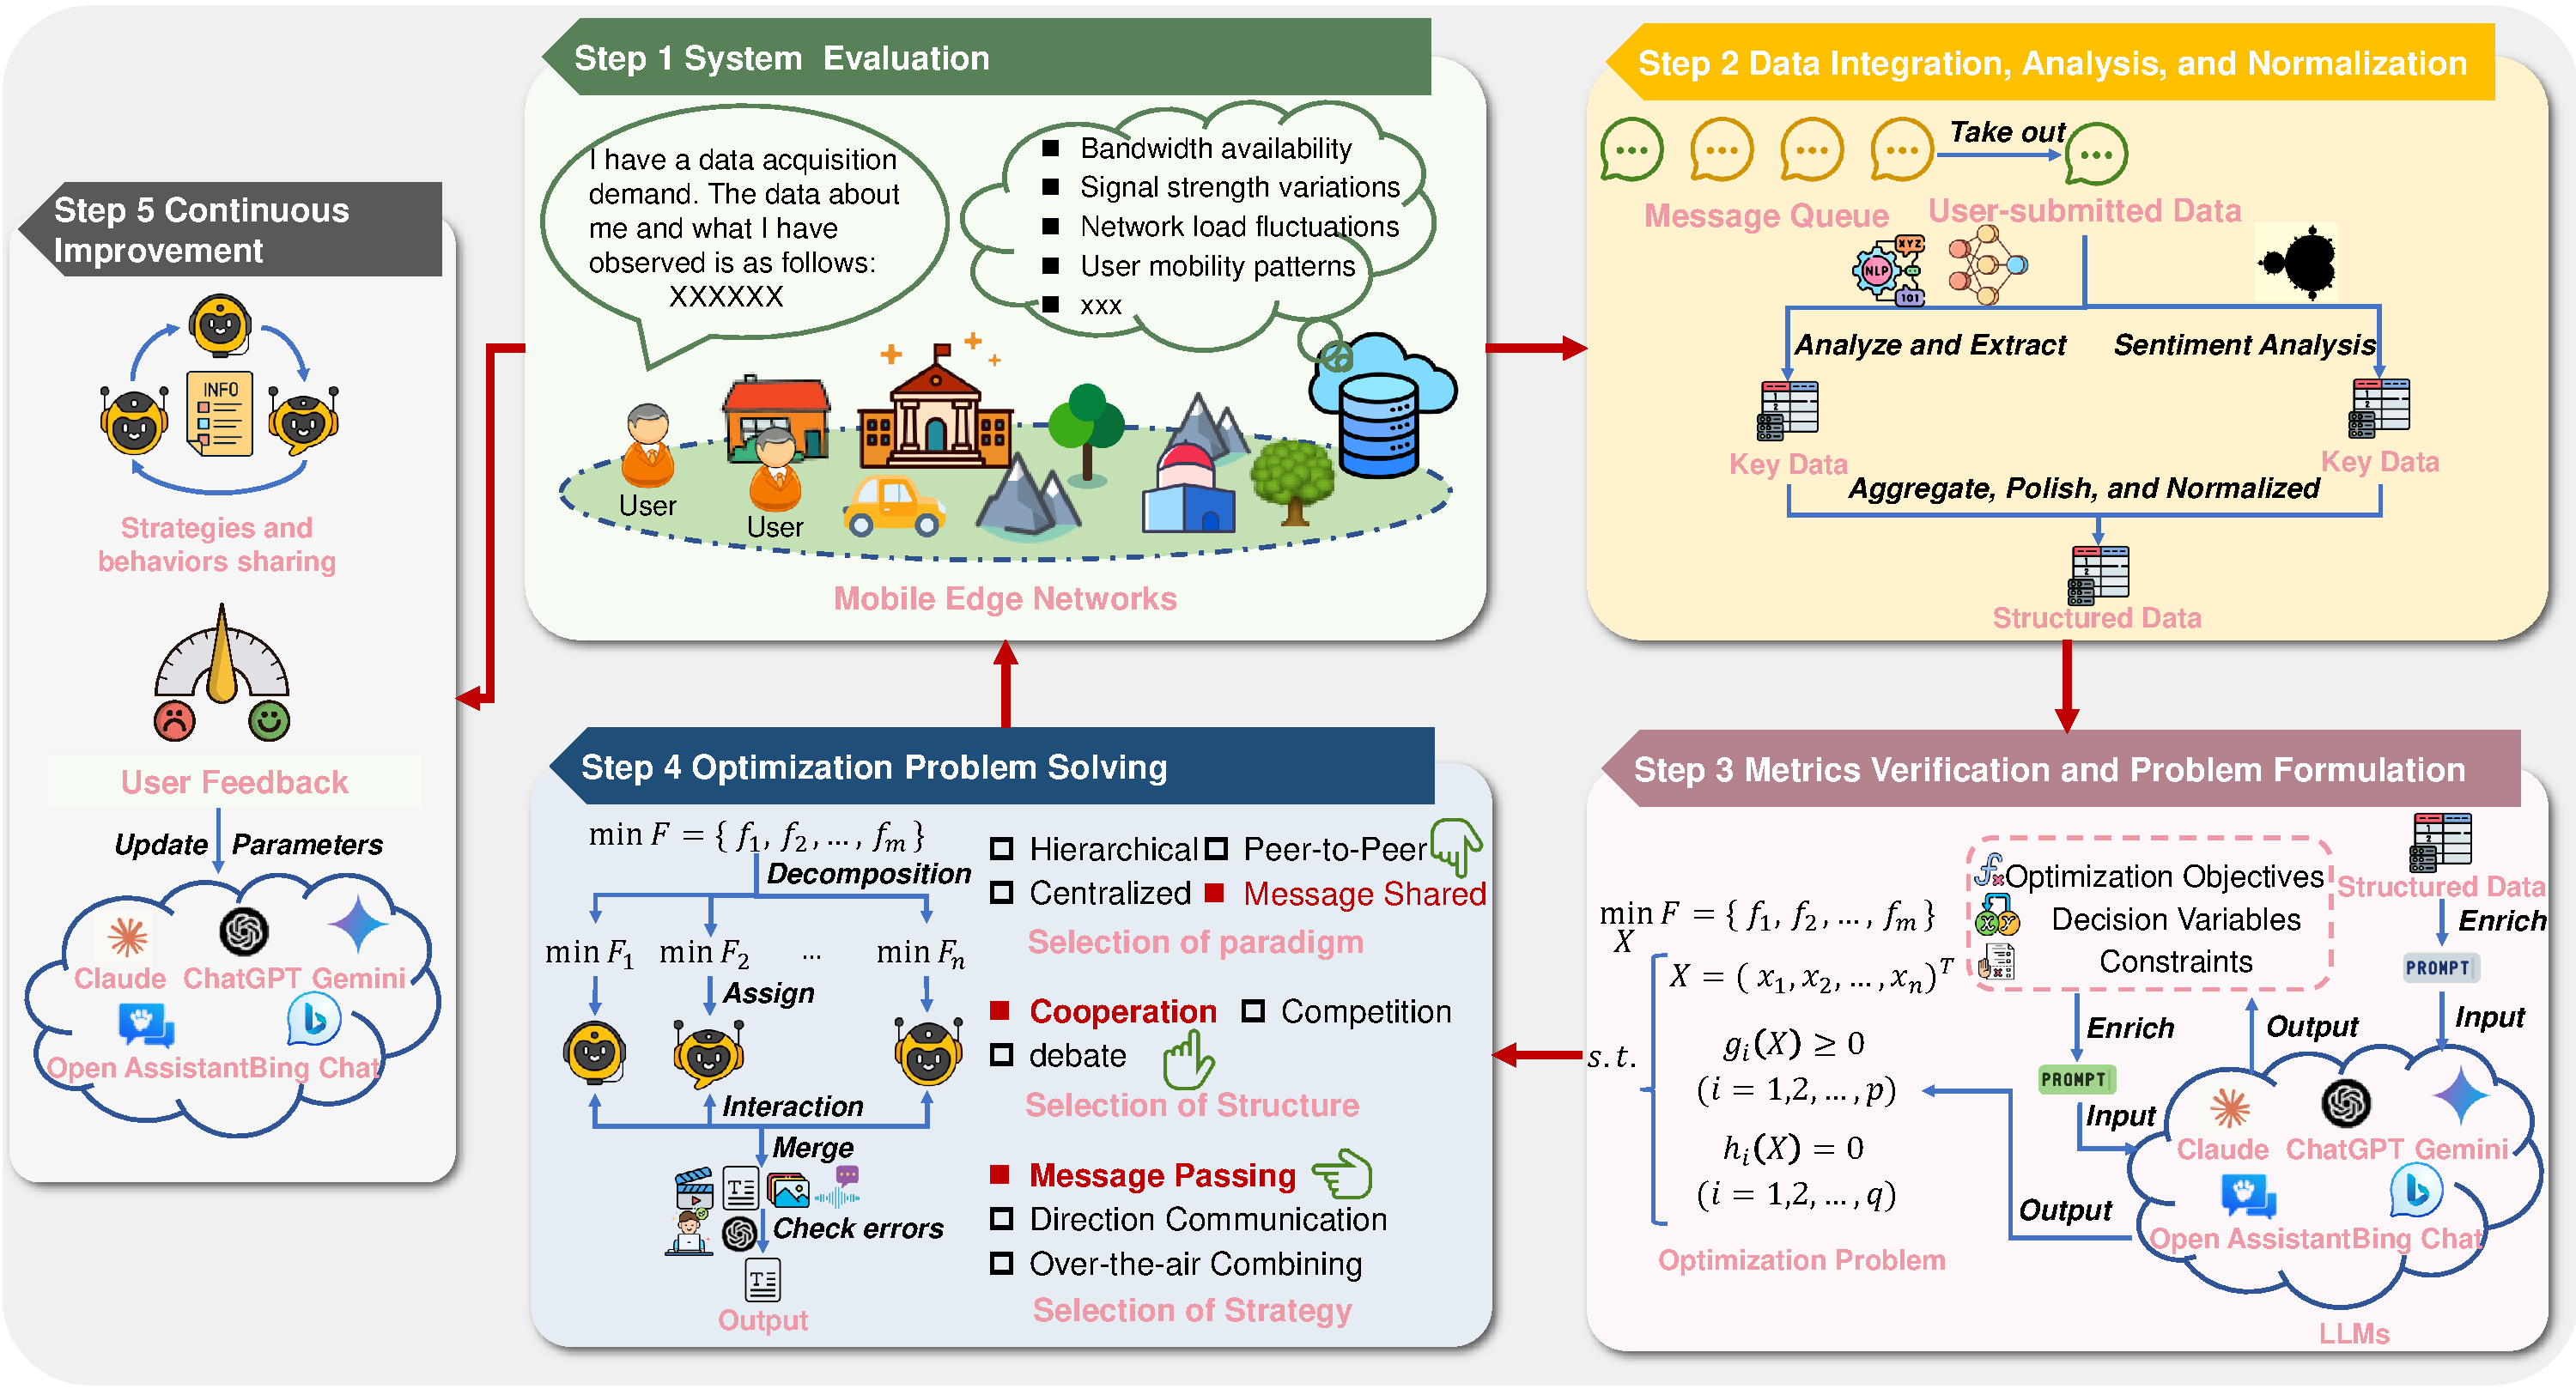
\includegraphics[width=6in]{figure/The Proposed Architecture.pdf}}
\caption{The framework of the proposed architecture. In step 1, a comprehensive evaluation is conducted to assess the current network conditions, predict task execution feasibility and efficiency, and optimize accordingly. In step 2, the GenAI-LLM interface module in the mobile edge server aggregates, analyze, and normalizes the data required by the GenAI-LLM. In step 3, the GenAI-LLM constructs the optimization problem based on the structured data. In step 4, interaction paradigm, structure, and strategy are determined. Moreover, the optimization problem is decomposed into several subproblems, each of which is assigned to an agent for execution. When the interaction among multiple agents ends, the output without errors and hallucinations is forwarded to the original user. In step 5, continuous improvement is conducted via knowledge sharing among agents and GenAI-LLM will update the its parameter based on user feedback and reinforcement learning techniques.}
\label{fig. sketch map}
\end{figure}

\newpage

{\setlength{\parskip}{0.3ex}
\begin{thebibliography}{100}%\bibitem[R1]{Near}
\bibitem [R1] {UDP} Y. Gu, and L. G. Robert, "UDT: UDP-based data transfer for high-speed wide area networks," \textit{Comp. Netw.}, vol. 51, no. 7, pp. 1777-1799, 2007.

\bibitem [R2] {MAVLink} S. Atoev, K. R. Kwon, S. H. Lee, and K. S. Moon, "Data analysis of the MAVLink communication protocol," \textit{Proc. {IEEE} {ICISCT}}, 2017.
    
\bibitem [R3] {Transformer} A. Vaswani, "Attention is all you need," \textit{Adv. Neural Inf. Process. Syst.}, 2017.
    
\bibitem [R4] {TextBlob} W. Aljedaani, F. Rustam, M.W. Mkaouer, A. Ghallab, V. Rupapara, P.B. Washington, E. Lee, and I. Ashraf, "Sentiment analysis on Twitter data integrating TextBlob and deep learning models: The case of US airline industry," \textit{Knowl.-Based Syst.}, vol. 255, pp. 109780.
    
\bibitem [R5] {VADER} C. Hutto, and G. Eric, "Vader: A parsimonious rule-based model for sentiment analysis of social media text," \textit{Proc. AAAI}, vol. 8. no. 1, 2014.
    
\bibitem [R6] {RAG1} P. Lewis, E. Perez, A. Piktus, F. Petroni, V. Karpukhin, N. Goyal, H. Küttler, M. Lewis, W.T. Yih, T. Rocktäschel, and S. Riedel, "Retrieval-augmented generation for knowledge-intensive nlp tasks," \textit{Adv. Neural Inf. Process. Syst.}, vol. 33, pp.9459-9474.

\bibitem [R7] {BCD} P. Tseng, "Convergence of a block coordinate descent method for nondifferentiable minimization," \textit{J. Optim. Theory Appl.}, vol. 109, pp.475-494.
    
\bibitem [R8] {policy gradient} J. Peters, and S. Schaal, "Reinforcement learning of motor skills with policy gradients," \textit{Neural Netw.}, vol. 21, no. 4, pp.682-697, 2008.
\end{thebibliography}

\end{document}
